% Methodology Design and Research Implementation (MAAI901 workshop report)
% Compile: tectonic main.tex   |   Overleaf: pdfLaTeX + BibTeX (default)
% numbers.tex is GENERATED by scripts/methodology_numbers.py; figures/ by scripts/methodology_figures.py.
\documentclass[12pt,a4paper]{article}

\usepackage[margin=1in]{geometry}
\usepackage[T1]{fontenc}
\usepackage{newtxtext,newtxmath}          % Times (text and maths)
\usepackage{setspace}
\usepackage{graphicx}
\usepackage{booktabs,array,tabularx,multirow}
\newcolumntype{Y}{>{\raggedright\arraybackslash}X}
\usepackage{caption}
\usepackage{enumitem}
\usepackage{xcolor}
\usepackage{microtype}
\usepackage[hidelinks]{hyperref}

\graphicspath{{figures/}}
\singlespacing
\setlength{\parskip}{0.35em}
\captionsetup{font=small,labelfont=bf,width=0.92\textwidth}
\setlist{nosep,leftmargin=*}
\renewcommand{\topfraction}{0.9}\renewcommand{\bottomfraction}{0.7}
\renewcommand{\textfraction}{0.07}\renewcommand{\floatpagefraction}{0.75}
\setcounter{topnumber}{3}\setcounter{totalnumber}{4}
\definecolor{signal}{RGB}{0,138,46}

% GENERATED by scripts/methodology_numbers.py from reports/tables, configs/base.yaml and
% reports/tables/methodology_inputs.json. Do not edit; rerun the script.

\newcommand{\augContrastMax}{1.1}
\newcommand{\augContrastMin}{0.9}
\newcommand{\augJpegMax}{95}
\newcommand{\augJpegMin}{50}
\newcommand{\augNoiseStdMax}{0.03}
\newcommand{\augRotationDeg}{180}
\newcommand{\augScaleMax}{1.2}
\newcommand{\augScaleMin}{0.8}
\newcommand{\augThickenProb}{0.3}
\newcommand{\backboneId}{facebook/dinov3-vitl16-pretrain-lvd1689m}
\newcommand{\benchEvalImgPerS}{98.5}
\newcommand{\benchGPU}{NVIDIA RTX 5000 Ada Generation}
\newcommand{\benchGPUs}{4}
\newcommand{\benchPeakMemGB}{5.5}
\newcommand{\benchTrainImgPerS}{22.5}
\newcommand{\benchTrainImgPerSLow}{64.9}
\newcommand{\bootstrapResamples}{1,000}
\newcommand{\ciLevelPct}{95}
\newcommand{\eceBins}{15}
\newcommand{\extrapEvalCap}{10,000}
\newcommand{\fallbackId}{facebook/dinov2-large}
\newcommand{\ftAmpDtype}{bfloat16}
\newcommand{\ftBackboneLR}{2\times 10^{-5}}
\newcommand{\ftBatch}{16}
\newcommand{\ftEMA}{0.999}
\newcommand{\ftEpochImages}{40,000}
\newcommand{\ftEpochs}{2}
\newcommand{\ftHeadLR}{1\times 10^{-3}}
\newcommand{\ftHoursPerRun}{1.0}
\newcommand{\ftLLRD}{0.8}
\newcommand{\ftLPEpochs}{30}
\newcommand{\ftLPQueries}{20,000}
\newcommand{\ftRealFractionPct}{50}
\newcommand{\ftTotalImages}{80,000}
\newcommand{\ftWarmupEpochs}{0.2}
\newcommand{\ftWeightDecay}{0.05}
\newcommand{\goldCeilingPct}{3}
\newcommand{\inputLongSide}{448}
\newcommand{\inputPadMultiple}{16}
\newcommand{\kneeEqualLengthPct}{2.32}
\newcommand{\medianCoordErrorPx}{2.4}
\newcommand{\nColourImages}{600}
\newcommand{\nColourNearHighlight}{0}
\newcommand{\nCoordPairs}{1,641}
\newcommand{\nFiguresTest}{370}
\newcommand{\nFiguresTrain}{1,296}
\newcommand{\nFiguresVal}{185}
\newcommand{\nGeometryFigures}{1,851}
\newcommand{\nGeometryProblems}{3,002}
\newcommand{\nGeometryTestDupTrain}{302}
\newcommand{\nGeometryTestImages}{601}
\newcommand{\nGeometryTestProblems}{601}
\newcommand{\nGeometryTestShareFigure}{327}
\newcommand{\nGeometryTrainProblems}{2,101}
\newcommand{\nGeometryValProblems}{300}
\newcommand{\nGoldAdjudicated}{3}
\newcommand{\nGoldRoundOne}{100}
\newcommand{\nGoldRoundTwo}{60}
\newcommand{\nHeldoutFigures}{660}
\newcommand{\nPgdpDiagrams}{5,000}
\newcommand{\nPgdpTest}{1,000}
\newcommand{\nPgdpTrain}{3,500}
\newcommand{\nPgdpVal}{500}
\newcommand{\nPgpsDiagrams}{4,000}
\newcommand{\nPgpsImagesGeometryTest}{515}
\newcommand{\nPgpsImagesPgdpTest}{558}
\newcommand{\nPoolFigures}{3,253}
\newcommand{\nQueriesGeometryTest}{11,319}
\newcommand{\nQueriesPgdpHeldout}{25,272}
\newcommand{\nQueriesPgpsPool}{66,019}
\newcommand{\nQueriesSynthExtrap}{60,000}
\newcommand{\nSeeds}{3}
\newcommand{\nTangentAssertedAll}{1}
\newcommand{\nTrainCollinear}{2,137}
\newcommand{\nTrainEqualAngle}{87}
\newcommand{\nTrainEqualLength}{315}
\newcommand{\nTrainMidpoint}{83}
\newcommand{\nTrainOnCircle}{1,337}
\newcommand{\nTrainParallel}{161}
\newcommand{\nTrainPerpBisector}{8}
\newcommand{\nTrainPerpendicular}{687}
\newcommand{\nTrainQueries}{37,846}
\newcommand{\nTrainTangent}{0}
\newcommand{\nUnmarkedGCollinear}{283}
\newcommand{\nUnmarkedGEqualLength}{11,171}
\newcommand{\nUnmarkedGOnCircle}{0}
\newcommand{\nUnmarkedGParallel}{1,534}
\newcommand{\nUnmarkedGPerpendicular}{1,244}
\newcommand{\nUnmarkedGTangent}{315}
\newcommand{\nUnmarkedPCollinear}{650}
\newcommand{\nUnmarkedPEqualLength}{37,121}
\newcommand{\nUnmarkedPOnCircle}{3}
\newcommand{\nUnmarkedPParallel}{4,635}
\newcommand{\nUnmarkedPPerpendicular}{3,847}
\newcommand{\nUnmarkedPTangent}{837}
\newcommand{\noneRatio}{3}
\newcommand{\ntsAngleDeg}{10}
\newcommand{\ntsLengthPct}{15}
\newcommand{\overlayHaloPx}{7}
\newcommand{\overlayRGB}{0, 200, 0}
\newcommand{\overlayWidthPx}{3}
\newcommand{\pctColourBlue}{85}
\newcommand{\pctColourGreenFamily}{1.0}
\newcommand{\pctColourRed}{53}
\newcommand{\pctConfirmedGCollinear}{99.8}
\newcommand{\pctConfirmedGEqualLength}{93.5}
\newcommand{\pctConfirmedGOnCircle}{99.9}
\newcommand{\pctConfirmedGParallel}{96.4}
\newcommand{\pctConfirmedGPerpendicular}{99.6}
\newcommand{\pctConfirmedGTangent}{0.0}
\newcommand{\pctConfirmedPCollinear}{99.9}
\newcommand{\pctConfirmedPEqualLength}{97.2}
\newcommand{\pctConfirmedPOnCircle}{100.0}
\newcommand{\pctConfirmedPParallel}{97.5}
\newcommand{\pctConfirmedPPerpendicular}{99.5}
\newcommand{\pctConfirmedPTangent}{0.0}
\newcommand{\pctCoordPairsOverTen}{12}
\newcommand{\pctGeometryPointsOutside}{0.09}
\newcommand{\pctGeometryTestDupTrain}{50}
\newcommand{\pctGeometryTestShareFigure}{54}
\newcommand{\pctGoldRoundOneFN}{8.8}
\newcommand{\pctGoldRoundOneFP}{5.1}
\newcommand{\pctGoldRoundTwoAdjFN}{0.0}
\newcommand{\pctGoldRoundTwoAdjFP}{0.0}
\newcommand{\pctGoldRoundTwoAdjStressFN}{0.0}
\newcommand{\pctGoldRoundTwoAdjStressFP}{3.8}
\newcommand{\pctGoldRoundTwoWeightedFN}{43.9}
\newcommand{\pctGoldRoundTwoWeightedFP}{0.1}
\newcommand{\pctNtsGeometry}{3.6}
\newcommand{\pctNtsGeometryFigures}{0.6}
\newcommand{\pctNtsPgdp}{0.6}
\newcommand{\pctNtsPgdpHeldout}{0.6}
\newcommand{\pctNtsPgps}{0.3}
\newcommand{\pctUnmarkedGCollinear}{8.8}
\newcommand{\pctUnmarkedGEqualLength}{96.5}
\newcommand{\pctUnmarkedGOnCircle}{0.0}
\newcommand{\pctUnmarkedGParallel}{89.0}
\newcommand{\pctUnmarkedGPerpendicular}{56.1}
\newcommand{\pctUnmarkedGTangent}{100.0}
\newcommand{\pctUnmarkedPCollinear}{6.7}
\newcommand{\pctUnmarkedPEqualLength}{93.0}
\newcommand{\pctUnmarkedPOnCircle}{0.1}
\newcommand{\pctUnmarkedPParallel}{90.1}
\newcommand{\pctUnmarkedPPerpendicular}{61.1}
\newcommand{\pctUnmarkedPTangent}{100.0}
\newcommand{\posWeightCap}{50}
\newcommand{\probeBatch}{256}
\newcommand{\probeEpochs}{50}
\newcommand{\probeLR}{1\times 10^{-3}}
\newcommand{\probePatience}{10}
\newcommand{\queryCap}{60}
\newcommand{\scalingSizes}{0, 1,000, 10,000, 50,000}
\newcommand{\seedList}{0, 1, 2}
\newcommand{\selftrainTau}{0.9}
\newcommand{\splitPctTest}{20}
\newcommand{\splitPctTrain}{70}
\newcommand{\splitPctVal}{10}
\newcommand{\synthCanvasPx}{512}
\newcommand{\synthCirclesMax}{2}
\newcommand{\synthExtrapPointsMax}{20}
\newcommand{\synthExtrapPointsMin}{12}
\newcommand{\synthExtrapSize}{1,000}
\newcommand{\synthInjectRate}{0.5}
\newcommand{\synthInjectedPassMinPct}{99.4}
\newcommand{\synthJitterPx}{1.0}
\newcommand{\synthMinSeparationPx}{30}
\newcommand{\synthPointsMax}{10}
\newcommand{\synthPointsMin}{4}
\newcommand{\synthPoolMax}{50,000}
\newcommand{\synthRandomPassEqualLengthPct}{11.2}
\newcommand{\synthRandomPassMaxPct}{4.3}
\newcommand{\synthRotationDeg}{5}
\newcommand{\synthSegmentsMax}{8}
\newcommand{\synthSegmentsMin}{3}
\newcommand{\synthUnlabelledSize}{2,000}
\newcommand{\tierTwoMinPositives}{200}
\newcommand{\tolCollinearPct}{1.19}
\newcommand{\tolEqualLengthPct}{10}
\newcommand{\tolOnCirclePct}{7.94}
\newcommand{\tolParallelDeg}{3.7}
\newcommand{\tolPerpendicularDeg}{3.7}
\newcommand{\tolTangentPct}{7.94}
\newcommand{\valleyParallelDeg}{2.56}
\newcommand{\valleyPerpendicularDeg}{2.03}
                           % \newcommand per measured quantity (generated)

\newcommand{\rel}[1]{\textsf{#1}}         % relation names
\newcommand{\evalunit}[1]{\texttt{#1}}    % evaluation units and file names
\newcommand{\Hone}{H\textsubscript{1}}
\newcommand{\Hzero}{H\textsubscript{0}}
\newcommand{\Htwo}{H\textsubscript{2}}

\title{Veridiagram: Methodology Design and Research Implementation}
\author{Parsa Hosseini}
\date{October 2026}

\begin{document}

% ---------------------------------------------------------------- 1. Title page
\begin{titlepage}
  \centering
  \vspace*{1.2cm}
  {\scshape\large Workshop: Methodology Design and Research Implementation\par}
  \vspace{1.6cm}
  {\LARGE\bfseries Veridiagram: Can a Vision Transformer Read the Geometry a Diagram Actually Contains?\par}
  \vspace{0.8cm}
  {\large\itshape A methodology for recognising formal geometric relations in textbook diagrams against coordinate-verified ground truth\par}
  \vspace{1.4cm}
  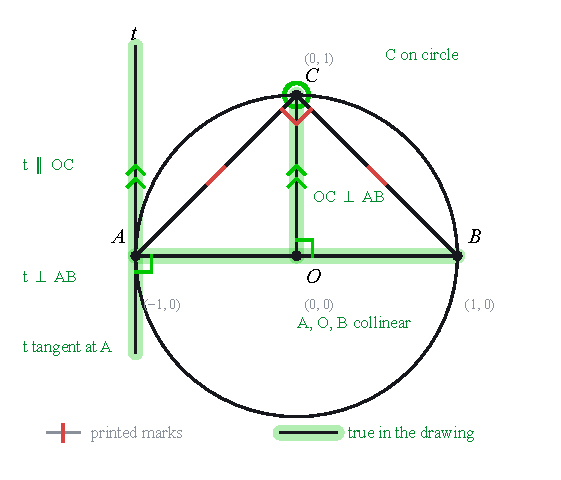
\includegraphics[width=0.62\textwidth]{fig_recap}\par
  \vspace{1.4cm}
  \begin{tabular}{@{}r@{\hspace{1.2em}}l@{}}
    \textsc{Course}     & MAAI901 Deep Learning for Visual Data \\
    \textsc{Instructor} & Dr.\ Milan Dordevic \\
    \textsc{Student}    & Parsa Hosseini \\
    \textsc{Student ID} & 7744547 \\
    \textsc{University} & University of Wollongong in Dubai \\
    \textsc{Date}       & October 2026 \\
  \end{tabular}
  \vfill
\end{titlepage}

% ---------------------------------------------------------------- 2. Table of contents
\tableofcontents
\clearpage

% ---------------------------------------------------------------- 3-11. Body (numbered as in the brief)
\setcounter{section}{2}
\section{Introduction and Recap of the Research Problem}
\label{sec:intro}

The previous workshop framed a study of how well a vision transformer reads the formal geometric relations contained in a textbook geometry diagram. Given a diagram and a named group of primitives (two segments, a point and a circle, or a segment and a circle), the task is to decide which relations hold between them: \rel{parallel}, \rel{perpendicular}, \rel{equal\_length}, \rel{on\_circle}, \rel{tangent} or \rel{collinear}. The defining choice is the reference against which correctness is judged. The datasets of the field record the relations an annotator chose to mark, usually because a symbol is printed in the figure \cite{lu2021intergps,zhang2022pgdp,zhang2023pgps}; this convention dates back to the first geometry solver \cite{seo2015geos}; this study instead takes the geometry of the drawing itself, measured from the coordinates of its points, as the ground truth, and compares it with the human annotation (Fig.~\ref{fig:recap}).

\begin{figure}[tbp]
  \centering
  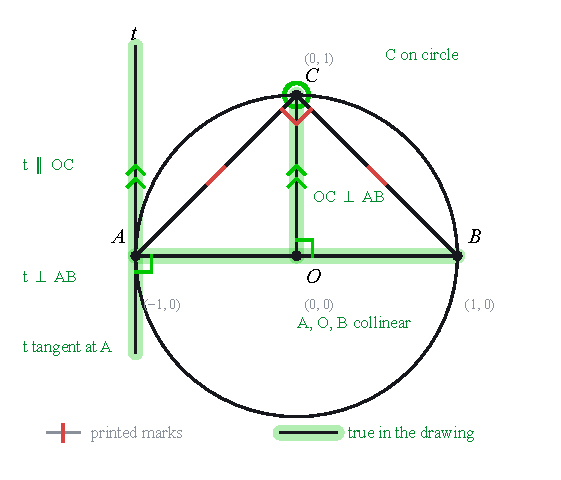
\includegraphics[width=0.6\textwidth]{fig_recap}
  \caption{One construction, two readings. Printed marks assert two relations (a right angle and two equal sides); the drawing satisfies six more that nobody marked (green). The verifier of Section~\ref{sec:preprocessing} labels all of them from the coordinates.}
  \label{fig:recap}
\end{figure}

The literature review identified four connected gaps. First, the ground truth in Geometry3K, PGDP5K and PGPS9K is the annotation, not the drawing, and a preliminary audit of the Geometry3K figures showed that most true relations are unmarked (\pctUnmarkedGParallel\% of the parallel pairs the drawings contain, \pctUnmarkedGPerpendicular\% of the perpendicular pairs, and all \nUnmarkedGTangent{} tangencies). Second, benchmark overlap hides generalisation: Geometry3K is split by problem rather than by figure, so \pctGeometryTestShareFigure\% of its test images share a figure with its training or validation split, and the three datasets reuse each other's images. Third, verifier-generated supervision, which lets AlphaGeometry train on unlimited correct synthetic data \cite{trinh2024alphageometry}, has never been applied to diagram perception. Fourth, perception is measured only indirectly, through problem answers \cite{zhang2024mathverse,gao2025gllava} or with annotated clauses in place of a parse \cite{zhang2023pgps}.

\paragraph{Problem statement.} \emph{Can a fine-tuned self-supervised vision transformer recognise the formal geometric relations that actually hold in a textbook diagram, when correctness is judged by a coordinate-based verifier rather than by human annotation; and does verifier-labelled synthetic data extend this ability to diagrams from an unseen source and to diagrams larger than any seen in training?}

\paragraph{Hypotheses.} \Hone: adding verifier-labelled synthetic diagrams to the real training data increases a fine-tuned vision transformer's macro-F1, measured against verifier labels, on (a) diagrams from an unseen source and (b) diagrams with more points than any training diagram, compared with training on real data alone at the same training budget. \Hzero: any difference in macro-F1 between the two training conditions is within the variation between random seeds. \Htwo: the same model scores substantially lower against human annotations than against verifier labels, and most of the difference comes from relations that hold in the drawing but are not marked.

This report turns that framing into a procedure. Section~\ref{sec:design} states the type of study and its variables; Sections~\ref{sec:dataset} and \ref{sec:preprocessing} describe the data and the pipeline that prepares it, including the verifier that produces the geometric labels; Sections~\ref{sec:model} and \ref{sec:training} give the model and the training plan with every setting; Section~\ref{sec:baselines} defines the comparisons; Section~\ref{sec:evaluation} the metrics and the decision rules for \Hone, \Hzero{} and \Htwo; and Section~\ref{sec:ethics} the ethical, bias and reproducibility provisions. Every quantity in the report is read from the project's configuration and data tables by a script, so that the text and the implementation cannot drift apart.

\section{Research Design}
\label{sec:design}

\subsection{Type of study}

This is an \emph{experimental, comparative classification study}. It is experimental because the quantity of interest is the effect of a controlled intervention, the composition of the training data, on a measured outcome, with everything else held fixed. It is comparative because the proposed method is judged against baselines and ablations trained under the same budget. It is a classification study because the model's output is a decision, per relation, about whether that relation holds for the queried primitives. Fig.~\ref{fig:design} shows the design.

\begin{figure}[tbp]
  \centering
  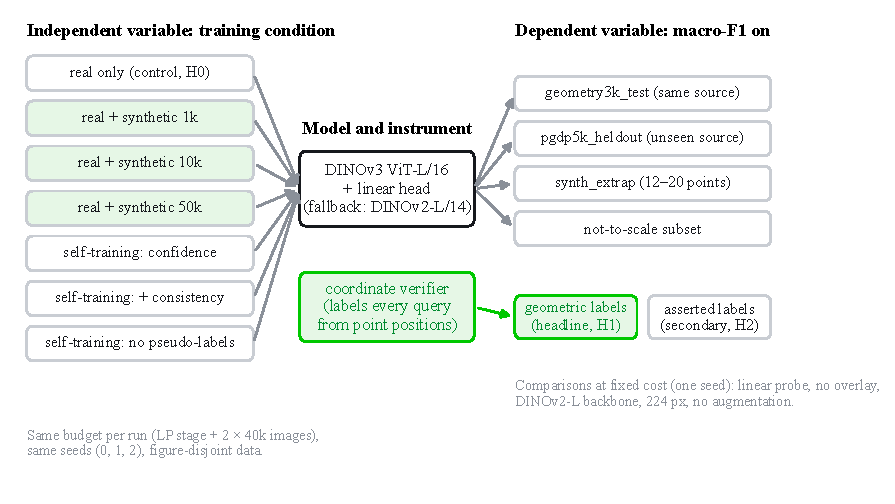
\includegraphics[width=\textwidth]{fig_design}
  \caption{Research design. Training conditions (left) vary the data; the model and the verifier are fixed; the outcome is macro-F1 on four evaluation sets against two label sets. Cheaper one-seed comparisons (bottom right) isolate design choices.}
  \label{fig:design}
\end{figure}

\subsection{Unit of analysis, inputs and outputs}

The unit of analysis is a \emph{query}: one diagram together with one tuple of its primitives. Segment pairs are queried for \rel{parallel}, \rel{perpendicular} and \rel{equal\_length}; point--circle pairs for \rel{on\_circle}; segment--circle pairs for \rel{tangent}; and point--segment triples for \rel{collinear}. The input to the model is the diagram image with the queried primitives highlighted (Section~\ref{sec:preprocessing}). The output is a six-dimensional vector of probabilities, one per relation, with an \emph{applicability mask} that excludes the relations a query kind cannot have: a segment pair can be both perpendicular and equal in length, but it cannot lie on a circle. A query with no positive relation is the \rel{none} case; it is represented as the all-zero vector rather than as a seventh class, so that multi-label queries remain expressible.

Primitive detection is out of scope by design: points, segments and circles come from the dataset annotations (Section~\ref{sec:dataset}). This isolates relation perception, the object of the hypotheses, from object detection, which the diagram-parsing literature already covers \cite{zhang2022pgdp}.

\subsection{Variables}

\paragraph{Independent variable.} The training condition. The primary contrast is \emph{real data only} against \emph{real data plus verifier-labelled synthetic diagrams}, at synthetic set sizes of \scalingSizes{} diagrams, every run at the same number of training images. A second contrast, within the self-training extension, is the pseudo-label filter: confidence alone, confidence with a deductive-consistency check, and a control that continues training without pseudo-labels.

\paragraph{Dependent variable.} Macro-F1 over the six relations, measured against the \emph{geometric} labels produced by the verifier, on four evaluation sets: the in-distribution test split, a held-out source never seen in training, a synthetic extrapolation set whose diagrams have \synthExtrapPointsMin--\synthExtrapPointsMax{} points (more than any training diagram), and the subset of real test diagrams flagged as not drawn to scale. The same predictions are also scored against the \emph{asserted} (human) labels; this second score is the outcome for \Htwo.

\paragraph{Controlled variables.} The backbone, resolution, augmentation, optimiser, schedule, training budget, random seeds, query enumeration and evaluation protocol are identical across the conditions of a contrast. Each design choice that could itself matter (backbone family, input resolution, augmentation, the highlight overlay) is varied once in a separate single-seed comparison (Section~\ref{sec:baselines}) rather than confounded with the main contrast.

\subsection{Why this design fits the hypotheses}

\Hone{} is a claim about a difference between two training conditions on two particular evaluation sets, so it needs a controlled contrast at equal budget, several seeds to estimate run-to-run variation, and evaluation sets that are provably disjoint from training (by figure, not by problem). \Hzero{} is the complement of \Hone{} under that same variation. \Htwo{} is a claim about two label sets on the same predictions, so every test query must carry both labels, which the two-label design provides. A purely predictive or applied design, which would optimise one model on one benchmark, could not separate the effect of the data from the effect of the labels; the comparative design does.

\section{Dataset Description}
\label{sec:dataset}

The study uses three public datasets of plane-geometry diagrams and one generated source (Table~\ref{tab:datasets}). The problem places five requirements on the data: real textbook diagrams; the coordinates of every annotated point, so that relations can be measured rather than assumed; human relation annotations, so that the measured truth can be compared with the marked one; a source independent of the training data; and a public licence. Together the four sources meet them: Geometry3K supplies the formal relation language with point positions, PGDP5K accurate positions and a mark-based annotation for the same figures plus a clean unseen source, PGPS9K a large pool of real diagrams, and the synthetic source the verifier-labelled data that \Hone{} is about. Geometry3K's two known defects, noisy coordinates and a problem-level split, are corrected in the pipeline (Section~\ref{sec:preprocessing}).

\begin{table}[tbp]
  \centering\small
  \caption{Data sources. Figure counts are after duplicate-image clustering (Section~\ref{sec:preprocessing}).}
  \label{tab:datasets}
  \begin{tabularx}{\textwidth}{@{}>{\hsize=.6\hsize}Y >{\hsize=1.0\hsize}Y >{\hsize=1.05\hsize}Y >{\hsize=.7\hsize}Y >{\hsize=1.65\hsize}Y@{}}
    \toprule
    Source & Size & Annotation & Coordinates & Role \\
    \midrule
    Geometry3K \cite{lu2021intergps} & \nGeometryProblems{} problems; \nGeometryFigures{} figures & formal language (91 predicates) & yes; offset, noisy & training, validation and in-distribution test \\
    PGDP5K \cite{zhang2022pgdp} & \nPgdpDiagrams{} diagrams & primitives, symbols, text, relation graph & yes; pixel-accurate & cleaner coordinates for shared figures; \nHeldoutFigures{} test figures as the unseen source \\
    PGPS9K \cite{zhang2023pgps} & \nPgpsDiagrams{} diagrams & textual clauses, solution programs & yes & pool of real diagrams used without labels (self-training) \\
    Synthetic & unlimited (\synthPoolMax{} generated) & verifier labels; injected constructions as marks & exact & verifier-labelled training data; extrapolation test \\
    \bottomrule
  \end{tabularx}
\end{table}

\subsection{Geometry3K}

Geometry3K \cite{lu2021intergps} contains \nGeometryProblems{} SAT-style problems, each with a diagram image, the problem text and a formal-language annotation. For the diagram, the annotation gives named points with positions (\texttt{point\_positions}), segments as pairs of point names (\texttt{line\_instances}), circles by their centre point, and relations as logic forms: \texttt{Parallel(Line(A,B), Line(C,D))}, \texttt{Perpendicular}, \texttt{Equals} of two \texttt{LengthOf} terms, \texttt{PointLiesOnCircle} and \texttt{PointLiesOnLine}. The published split is by problem (\nGeometryTrainProblems{} / \nGeometryValProblems{} / \nGeometryTestProblems); the \nGeometryProblems{} problems use only \nGeometryFigures{} distinct figures. The images are PNG with a transparent background, accompanied by a copy in which every annotated point is drawn as a red dot. Three defects matter for this study. The coordinates are not image pixels but carry a per-diagram translation, which the pipeline recovers from the red-dot image. Against PGDP5K's pixel re-annotation of the same images (\nCoordPairs{} image pairs) the median point error is \medianCoordErrorPx{} px, but \pctCoordPairsOverTen\% of the pairs have at least one point more than 10 px off. And \nGeometryTestDupTrain{} of the \nGeometryTestImages{} test images (\pctGeometryTestDupTrain\%) are exact copies of a training image, while \nGeometryTestShareFigure{} (\pctGeometryTestShareFigure\%) share a figure with the training or validation split.

\subsection{PGDP5K}

PGDP5K \cite{zhang2022pgdp} contains \nPgdpDiagrams{} diagrams (\nPgdpTrain{} / \nPgdpVal{} / \nPgdpTest), of which 1,813 are Geometry3K images re-annotated and the rest come from textbooks. The annotation is at the level of primitives in pixel coordinates (points, the longest segment of each line, circles with centre and radius), symbols with a class (perpendicular mark, one to four tick bars, one to three parallel arrows, angle arcs, text) and a relation graph linking symbols to primitives and points to the lines and circles they lie on. Asserted relations are read from the marks: a right-angle symbol asserts \rel{perpendicular} between its two lines, tick marks of the same class assert \rel{equal\_length}, parallel arrows of the same class assert \rel{parallel}, and the incidence relations give \rel{on\_circle} and \rel{collinear}. No tangent is marked anywhere in the three real datasets: \nTangentAssertedAll{} assertion exists in total. The \nHeldoutFigures{} PGDP5K test figures with no Geometry3K copy form the \emph{held-out source}.

\subsection{PGPS9K}

PGPS9K \cite{zhang2023pgps} contains \nPgpsDiagrams{} diagrams in the same primitive format as PGDP5K, paired with 9,022 problems; 1,738 of its diagrams are Geometry3K images, and it also contains \nPgpsImagesGeometryTest{} Geometry3K test images and \nPgpsImagesPgdpTest{} PGDP5K test images, so it can only serve as an unlabelled pool after those copies are removed. Its labels are not used for training; they are unsealed only post hoc to measure pseudo-label precision (Section~\ref{sec:evaluation}).

\subsection{Synthetic diagrams}

Because the verifier can label any diagram whose coordinates are known, generated diagrams provide unlimited training labels, can be made larger than any real diagram, and can contain relations that are rare in textbooks. The generator (Section~\ref{sec:preprocessing}) produces a training pool of \synthPoolMax{} diagrams with \synthPointsMin--\synthPointsMax{} points, of which the first 1,000 and 10,000 are nested subsets for the scaling contrast; an extrapolation pool of \synthExtrapSize{} diagrams with \synthExtrapPointsMin--\synthExtrapPointsMax{} points; and an unlabelled pool of \synthUnlabelledSize{} diagrams whose coordinates are sealed. Fig.~\ref{fig:examples} shows real and synthetic examples with their query overlays.

\begin{figure}[tbp]
  \centering
  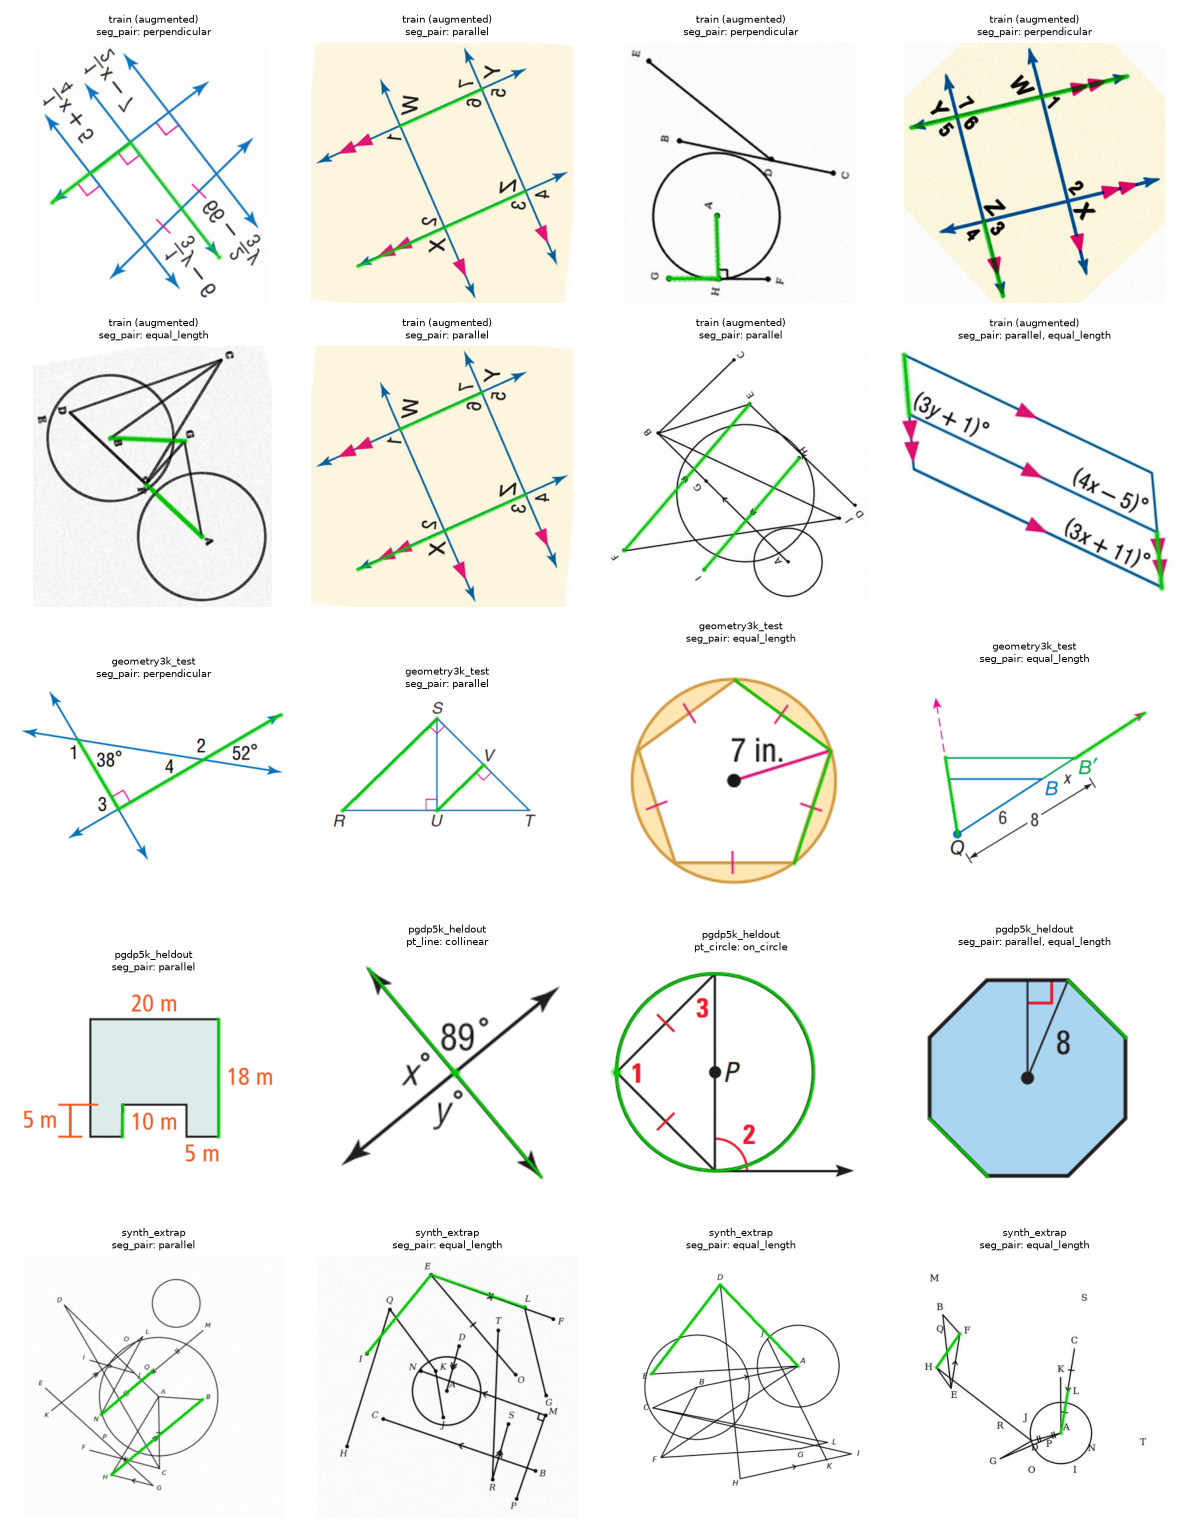
\includegraphics[width=\textwidth]{dataset_examples}
  \caption{Queries from each unit: augmented training queries (top two rows), in-distribution test, held-out source and synthetic extrapolation. The queried primitives are highlighted in green; everything else is the original image.}
  \label{fig:examples}
\end{figure}

\subsection{Inputs, targets and access}

The model input is one image and one query; the target is the six-way multi-label vector with its applicability mask, in two versions, \emph{asserted} and \emph{geometric}. Asserted positives in the training split, counted once per figure, are \nTrainParallel{} \rel{parallel}, \nTrainPerpendicular{} \rel{perpendicular}, \nTrainEqualLength{} \rel{equal\_length}, \nTrainOnCircle{} \rel{on\_circle}, \nTrainCollinear{} \rel{collinear} and \nTrainTangent{} \rel{tangent}; three further relation types available in the annotations (\rel{midpoint} \nTrainMidpoint, \rel{equal\_angle} \nTrainEqualAngle, \rel{perp\_bisector} \nTrainPerpBisector) fall below the pre-set inclusion threshold of \tierTwoMinPositives{} positives and are excluded. All three datasets are public under MIT licences through the authors' repositories or Hugging Face dataset cards, contain no personal data, and are small enough (under 10,000 distinct real diagrams, about 1 GB) to process on one machine; the archives are verified by SHA-256 on download.

\section{Data Preprocessing and Preparation}
\label{sec:preprocessing}

Fig.~\ref{fig:pipeline} shows the pipeline from raw annotations to training batches. Each step is a command in the project repository, and the steps run in the order given here.

\begin{figure}[tbp]
  \centering
  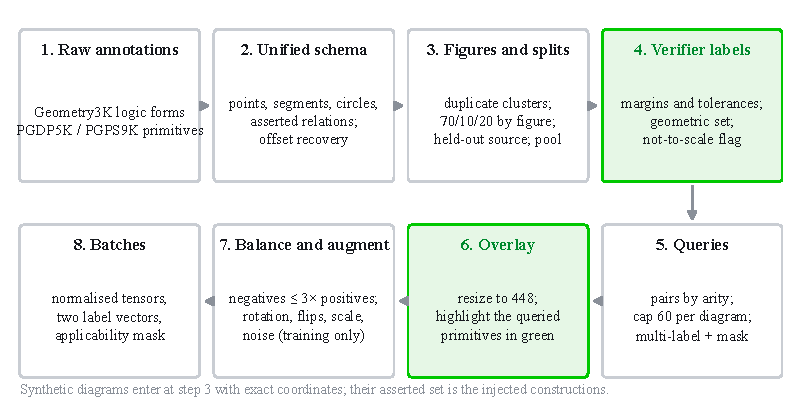
\includegraphics[width=\textwidth]{fig_pipeline}
  \caption{The data pipeline. Green steps are the two that distinguish this study: the verifier that produces the geometric labels, and the overlay that turns a query into an image.}
  \label{fig:pipeline}
\end{figure}

\subsection{Unified schema and loaders}

One loader per source converts the raw annotation into a single \texttt{Diagram} record: image path and size; points as name $\to$ pixel coordinates (origin top-left); segments as pairs of point names; lines as collinear point groups; circles as centre, radius and the points on them; and the asserted relations with their type and arguments. For Geometry3K, whose positions carry a per-diagram translation, the loader recovers the offset by matching the positions to the red dots in the point-annotated image (all points matched in 2,985 of 3,001 diagrams with points; the remainder are flagged). Geometry3K stores no numeric radius, so the loader uses the median distance from the centre to its annotated on-circle points. Every relation name is mapped to one of the six target relations by a fixed table (for example \texttt{PointLiesOnCircle} $\to$ \rel{on\_circle}; a right-angle symbol $\to$ \rel{perpendicular}), so that all sources share one definition. A sanity check confirms that annotated points fall inside the image (\pctGeometryPointsOutside\% of Geometry3K points do not, after offset recovery; none in the other sources).

\subsection{Figure clustering and splits}

Because the same figure recurs across problems and across datasets, the unit of splitting is the \emph{figure}, a cluster of duplicate images. Candidates are found by a 64-bit difference hash within a small Hamming distance and confirmed by near-identical pixels at low resolution or by the overlap of their ink together with agreement of the labelled point names; low-resolution similarity alone was found to match different simple triangles and is not enough. The \nGeometryFigures{} Geometry3K figures are re-split \splitPctTrain/\splitPctVal/\splitPctTest{} with a fixed seed, stratified by whether the figure contains a circle, into \nFiguresTrain{} / \nFiguresVal{} / \nFiguresTest{} figures. Where PGDP5K re-annotated a figure, its pixel-accurate annotation replaces Geometry3K's; otherwise Geometry3K's is kept. The held-out source is the \nHeldoutFigures{} PGDP5K test figures that have no Geometry3K copy, and the self-training pool is the \nPoolFigures{} PGPS9K figures that appear in no validation or test set (only the ones outside the training split are pseudo-labelled). A test asserts that no diagram and no figure appears in two units.

\subsection{Geometric labelling by the verifier}
\label{sec:verifier}

The verifier decides every relation from coordinates in double precision. Each check returns the raw \emph{margin}, a scale-free quantity that measures how far the primitives are from satisfying the relation, and the decision is the margin compared with a fixed tolerance (Table~\ref{tab:verifier}). Relative tolerances make the checks independent of image size; for \rel{collinear} the distance is normalised by the \emph{diagram scale}, the diagonal of the bounding box of all points. Two refinements came from the gold-set audit below: a segment with both endpoints on the circle is a chord, not a tangent, and the tangency point may sit at a segment's end; and two coincident lines are not counted as parallel.

\begin{table}[tbp]
  \centering\small
  \caption{Relation checks. $\theta$ is the angle between two segments, $|s|$ a segment length, $c$ and $r$ a circle's centre and radius, $d(\cdot)$ a point-to-line distance, $D$ the diagram scale. A query is positive when its margin is at most the tolerance.}
  \label{tab:verifier}
  \begin{tabular}{@{}l l l l@{}}
    \toprule
    Relation & Margin & Tolerance & Origin of the value \\
    \midrule
    \rel{parallel}      & $|\sin\theta|$                              & $\sin(\tolParallelDeg^\circ)$       & valley at \valleyParallelDeg$^\circ$, widened after gold round 1 \\
    \rel{perpendicular} & $|\cos\theta|$                              & $\sin(\tolPerpendicularDeg^\circ)$  & valley at \valleyPerpendicularDeg$^\circ$, widened after gold round 1 \\
    \rel{equal\_length} & $\bigl||s_1|-|s_2|\bigr| / \max(|s_1|,|s_2|)$ & \tolEqualLengthPct\%               & knee at \kneeEqualLengthPct\%, widened after gold round 1 \\
    \rel{on\_circle}    & $\bigl||p-c|-r\bigr| / r$                   & \tolOnCirclePct\%                   & density valley \\
    \rel{tangent}       & $|d(c, s)-r| / r$, foot on $s$, not a chord & \tolTangentPct\%                    & equals \rel{on\_circle} (no asserted tangents) \\
    \rel{collinear}     & $|(b-a)\times(p-a)| / (|b-a|\,D)$           & \tolCollinearPct\% of $D$           & density valley \\
    \bottomrule
  \end{tabular}
\end{table}

\paragraph{Calibration.} For each relation, the margin is computed for every candidate query in the training split and split by whether the query is asserted (Fig.~\ref{fig:tolerance}). The initial tolerance is the valley between the two modes of the smoothed log-margin density, or, where there is no valley (\rel{equal\_length}), the knee of the asserted cumulative distribution.

\begin{figure}[tbp]
  \centering
  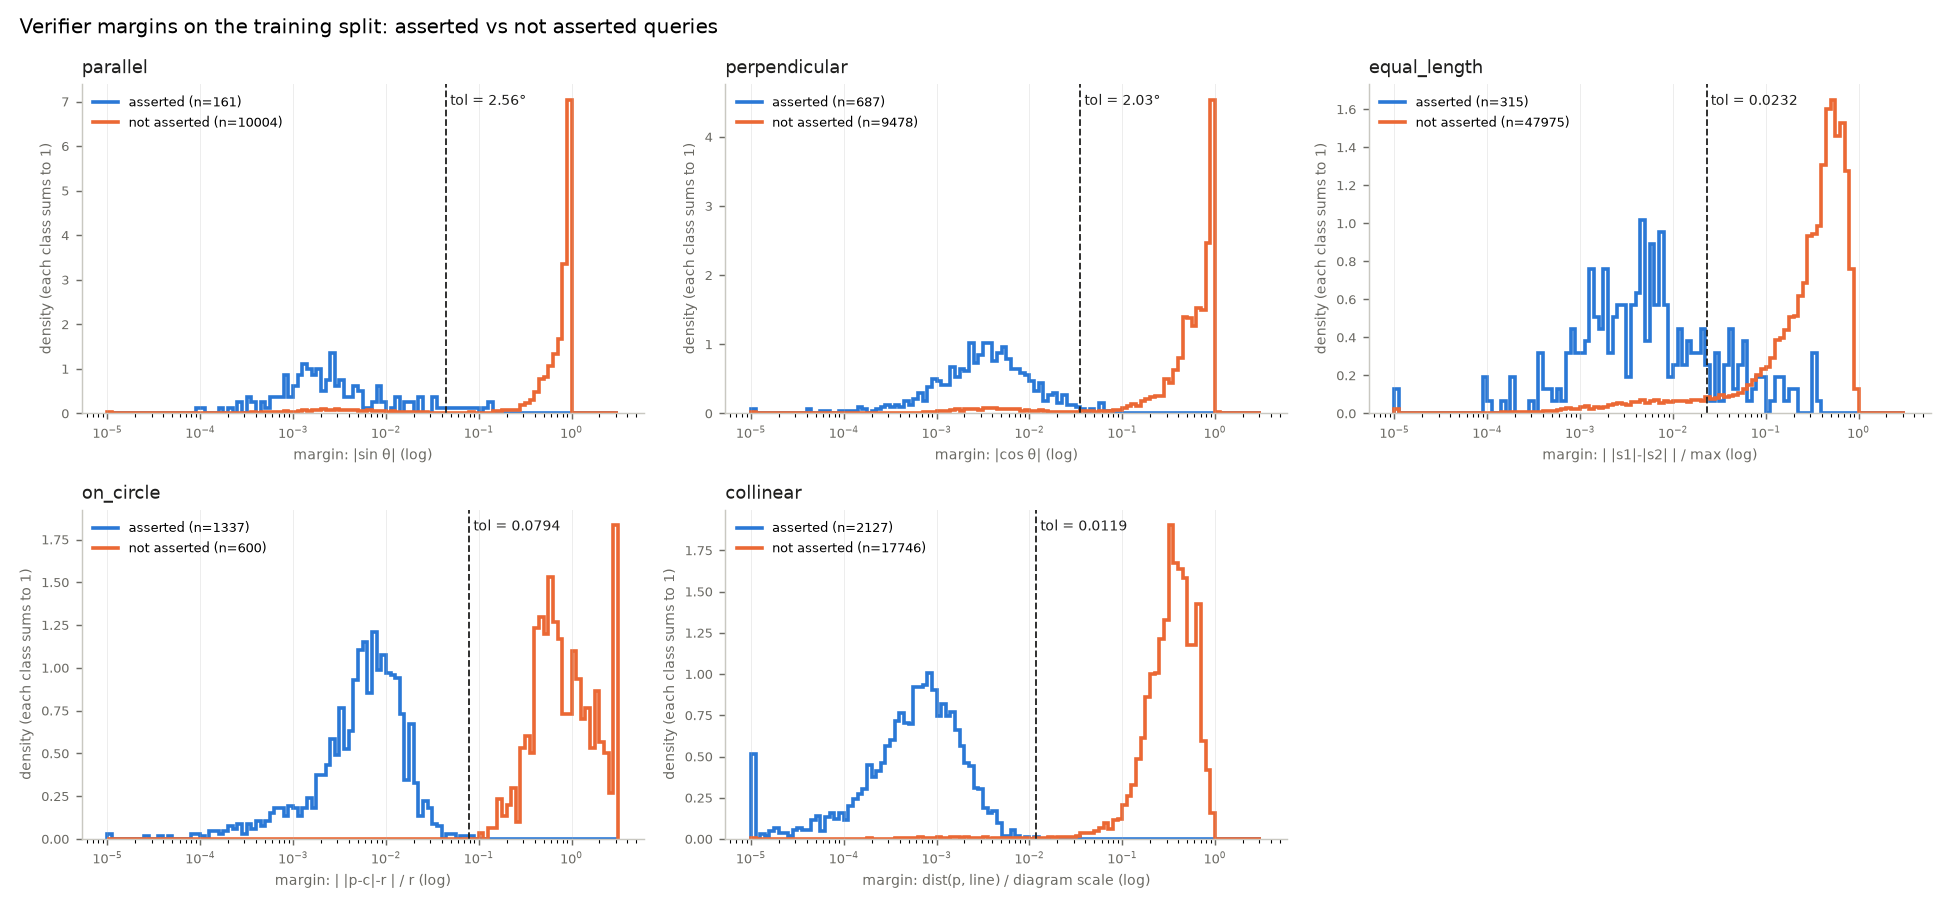
\includegraphics[width=\textwidth]{tolerance_all}
  \caption{Margin distributions on the training split, asserted queries against the rest, with the calibrated thresholds. The annotation and the drawing agree for most relations; the overlap for \rel{equal\_length} is the reason its tolerance was set by a human audit rather than by the histogram.}
  \label{fig:tolerance}
\end{figure}

\paragraph{Gold-set validation.} Because the verifier is the measuring instrument of the whole study, its agreement with a human reading of the diagram is checked on a gold set labelled by eye, without access to the annotation, with a pre-registered ceiling of \goldCeilingPct\% for both the false-positive and the false-negative rate. Round~1 (\nGoldRoundOne{} queries, enriched near the tolerances) failed the gate (FP \pctGoldRoundOneFP\%, FN \pctGoldRoundOneFN\%): the eye accepts more than the histogram valleys, so the angle tolerances were widened to \tolParallelDeg$^\circ$ and the length tolerance to \tolEqualLengthPct\%, within the range consistent with every round-1 label. Because round~1 informed the revision, the gate is decided on a fresh round~2 (\nGoldRoundTwo{} new queries plus a blind re-check of round-1 disagreements mixed with as many agreements), scored with population weights that undo the near-tolerance oversampling. The raw round-2 rates were FP \pctGoldRoundTwoWeightedFP\% and FN \pctGoldRoundTwoWeightedFN\%, the latter driven by \nGoldAdjudicated{} items that the labeller, on re-inspection, confirmed as slips (a radius labelled tangent; sides 24\% apart labelled equal); they are recorded in an adjudication file with the raw labels untouched. The adjudicated weighted rates are FP \pctGoldRoundTwoAdjFP\% and FN \pctGoldRoundTwoAdjFN\%, which passes the gate; the unweighted stress rates are reported alongside (FP \pctGoldRoundTwoAdjStressFP\%, FN \pctGoldRoundTwoAdjStressFN\%).

\paragraph{Labels and flags.} With the tolerances fixed, the verifier enumerates every candidate query of every diagram and writes the \emph{geometric} relation set with its margins, next to the \emph{asserted} set. A diagram is flagged \emph{not to scale} when any asserted relation fails its check by a large margin (more than \ntsAngleDeg$^\circ$ for angles or \ntsLengthPct\% for lengths); flagged diagrams stay in the data and are evaluated as a separate category. The flag fires on \pctNtsGeometryFigures\% of the curated Geometry3K figures, \pctNtsPgdp5k\% of PGDP5K and \pctNtsPgps9k\% of PGPS9K.

\subsection{Query enumeration and labels}

Candidate queries are enumerated per diagram by arity: all segment pairs, all point--circle pairs, all segment--circle pairs, and all point--segment triples, excluding nested sub-segments of one drawn line. To bound the dataset, at most \queryCap{} queries per diagram are kept: in the training unit every positive is kept and negatives fill the remainder; in evaluation units the sample is uniform, so the natural ratio of positives to negatives is preserved. Each query carries two six-dimensional label vectors (geometric and asserted) and the applicability mask of its kind. The resulting units hold \nTrainQueries{} training queries, \nQueriesGeometryTest{} in-distribution test queries, \nQueriesPgdpHeldout{} held-out-source queries and \nQueriesSynthExtrap{} extrapolation queries, of which \extrapEvalCap{} evenly spaced ones are evaluated.

\subsection{Overlay rendering and normalisation}

A query becomes an image by drawing the queried primitives on the diagram in a fixed highlight colour, RGB (\overlayRGB), \overlayWidthPx{} px wide with a semi-transparent halo of \overlayHaloPx{} px; a point is drawn as a filled marker and a circle is traced. Everything else is left unchanged, and a unit test asserts that no pixel outside the highlighted primitives is altered. The colour was chosen by measurement: in \nColourImages{} sampled real diagrams, red, orange and cyan ink occur in \pctColourRed\%, 68\% and 14\% of images respectively and blue in \pctColourBlue\%, whereas no image (\nColourNearHighlight{} of \nColourImages) contains a colour within distance 80 of the highlight, so the highlight cannot be confused with ink. The image is first resized so that its long side is \inputLongSide{} px with the aspect ratio preserved, then the overlay is drawn (so the highlight has the same width in every input), then the image is padded with white to a multiple of \inputPadMultiple{} px, the backbone's patch size, and normalised with the backbone's mean and standard deviation. Overlays are cached to disk as PNG, keyed by diagram and query. The dataset object returns, per query, the normalised tensor, both label vectors, the mask and metadata; batches of \ftBatch{} are padded with normalised white to the largest image in the batch.

\subsection{Negative balancing and class weights}

Negatives dominate the natural query distribution. For training only, the all-negative queries of each query kind are downsampled to at most \noneRatio$\times$ the number of positive queries of that kind, so that the head does not collapse to \rel{none}. In addition the loss weights each relation's positives by the ratio of applicable negatives to positives in the training split, capped at \posWeightCap{}. Evaluation units keep the natural ratio.

\subsection{Relation-preserving augmentation}

Training images are augmented after the overlay, so the highlight transforms with the diagram: rotation by up to $\pm\augRotationDeg^\circ$, horizontal and vertical flips, scaling of the ink box by \augScaleMin--\augScaleMax{} (as a crop and resize capped at the input size, so nothing is cut), line thickening by a $3\times3$ minimum filter with probability \augThickenProb, Gaussian noise with standard deviation up to \augNoiseStdMax, JPEG re-encoding at quality \augJpegMin--\augJpegMax, and contrast change by \augContrastMin--\augContrastMax. Shear and perspective are excluded because they break parallelism and length equality, and therefore the labels.

\subsection{Synthetic diagram generation}

The generator samples \synthPointsMin--\synthPointsMax{} points on a \synthCanvasPx{} px canvas with a minimum separation of \synthMinSeparationPx{} px, \synthSegmentsMin--\synthSegmentsMax{} segments and up to \synthCirclesMax{} circles. Each construction step, with probability \synthInjectRate, injects a relation exactly (a segment parallel or perpendicular to another, a segment of equal length, a point on a segment or on a circle, a tangent at a circle point; \rel{tangent} is weighted double because real data has no positives), otherwise it adds a random point or segment. The injected constructions form the synthetic \emph{asserted} set and are drawn as textbook marks. The diagram is then rotated by up to \synthRotationDeg$^\circ$ and every coordinate is jittered by Gaussian noise of \synthJitterPx{} px, so that the \emph{geometric} truth is decided by the verifier rather than by the construction, exactly as for real data. Rendering varies line width, font, label offset and, with some probability, scan noise and JPEG artefacts (Fig.~\ref{fig:synthetic}). A verification pass confirms that injected relations pass their checks in at least \synthInjectedPassMinPct\% of cases while random candidates pass in at most \synthRandomPassMaxPct\% (\synthRandomPassEqualLengthPct\% for \rel{equal\_length}, whose chance rate is higher). Every diagram is a pure function of the seed and its index, so the pools regenerate bit-for-bit on any machine. The extrapolation pool uses \synthExtrapPointsMin--\synthExtrapPointsMax{} points; the unlabelled pool's annotation is sealed with a SHA-256 digest before any experiment and opened only for post-hoc analysis.

\begin{figure}[tbp]
  \centering
  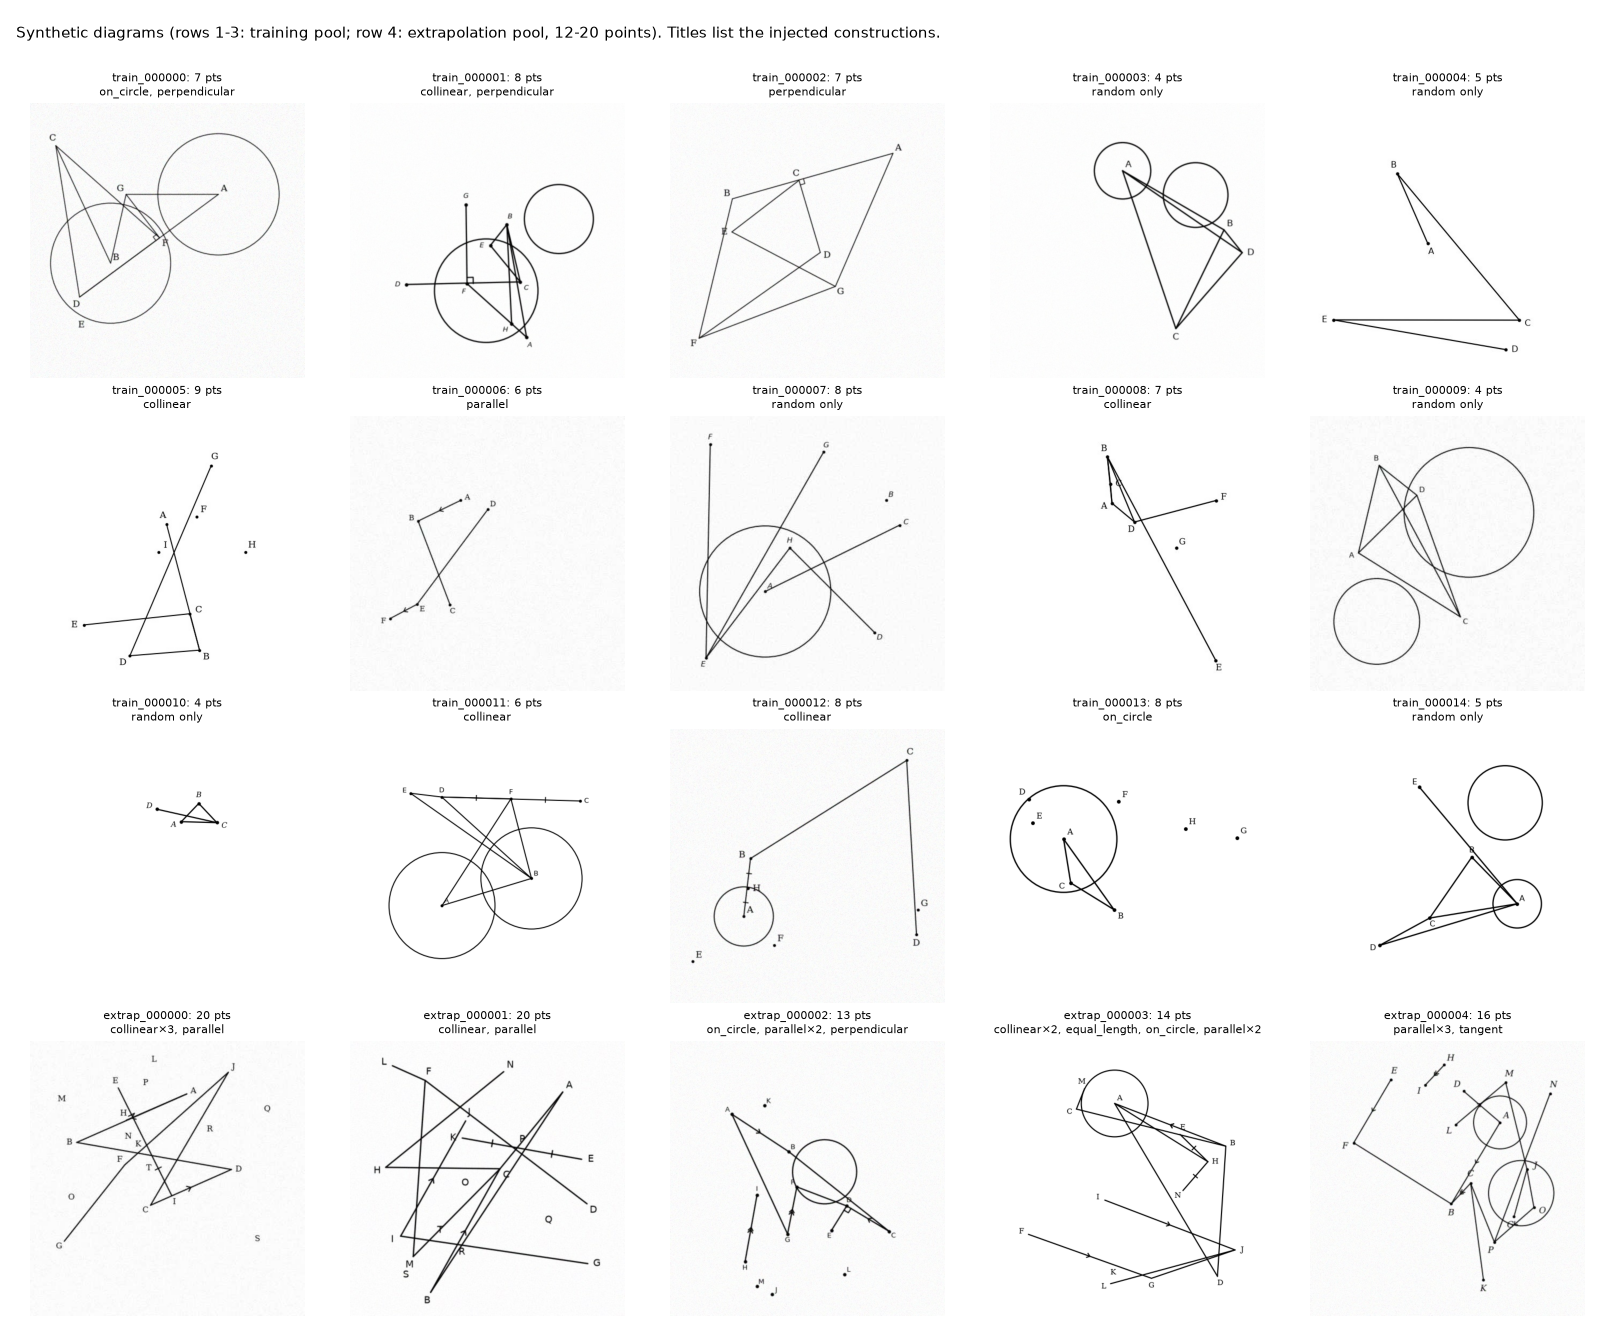
\includegraphics[width=\textwidth]{synthetic_examples}
  \caption{Synthetic diagrams from the training pool, with the injected relations drawn as marks and the rendering style varied.}
  \label{fig:synthetic}
\end{figure}

\section{Proposed Model or Transformer}
\label{sec:model}

\subsection{Backbone}

The proposed backbone is \textbf{DINOv3 ViT-L/16} \cite{simeoni2025dinov3}, loaded from the Hugging Face hub as \texttt{\backboneId}. It is a vision transformer \cite{dosovitskiy2021vit} with 24 layers, 1,024-dimensional tokens, $16\times16$ pixel patches and four register tokens \cite{darcet2024registers}, about 300 million parameters, trained without labels by self-distillation on a curated set of about 1.7 billion images and distilled from a 7-billion-parameter teacher. Its role in the study is that of a feature extractor that is fine-tuned end to end: the image with the highlighted query enters as a sequence of patch tokens, and the relation decision is read from the output tokens.

Four properties make it suitable, each tied to a property of the data. Global self-attention relates every patch to every other patch in every layer, whereas a convolutional network such as ResNet \cite{he2016resnet} connects distant regions only in its deepest layers; this matters because a relation is a property of primitives that may lie far apart in the image. Self-supervised training on images alone yields dense, stroke-level features, and DINOv3's \emph{Gram anchoring} is designed to keep the patch-level features from degrading over long training \cite{simeoni2025dinov3}; caption-aligned encoders such as CLIP \cite{radford2021clip} learn what captions describe, and captions do not describe angles. The model accepts inputs of varying size, so diagrams are processed at a resolution that keeps thin lines and small marks without distortion. And its features are strong when frozen \cite{oquab2024dinov2,simeoni2025dinov3}, which allows a frozen-feature baseline on the small real training set (\nFiguresTrain{} figures) as well as full fine-tuning.

\textbf{DINOv2 ViT-L/14} \cite{oquab2024dinov2} (\texttt{\fallbackId}) is the named fallback and comparison: it is peer-reviewed, whereas DINOv3 is at present a preprint, and it is run under the identical recipe in one comparison (Section~\ref{sec:baselines}). At the same input size its 14-pixel patches yield 1,024 patch tokens against 784 for DINOv3, a difference the comparison must keep in mind. The backbone identifier is a single configuration value, so switching between them changes nothing else.

\subsection{Feature pooling and head}

From the backbone's output the model drops the register tokens and forms a pooled feature by concatenating the CLS token with the mean of the patch tokens (2,048 dimensions), so that both a global summary and the average local evidence reach the head. The head is a LayerNorm followed by one linear layer with six outputs and a sigmoid per output: a multi-label classifier, because a segment pair can be both perpendicular and equal in length. The loss is binary cross-entropy over the applicable relations only (the mask zeroes the others), with the per-relation positive weights of Section~\ref{sec:preprocessing}. Gradient checkpointing \cite{chen2016checkpointing} is enabled so that the full fine-tune fits in a few gigabytes of GPU memory at \inputLongSide{} px. Every choice named in this section is one entry of the configuration file summarised in Table~\ref{tab:config}.

\subsection{Query-as-tokens variant}

To test whether the highlight overlay, rather than any other part of the design, is what makes the task learnable, one comparison model receives the query not as a highlight but as tokens: the query kind and the point names, hashed to token indices, are embedded and projected to a single query vector that cross-attends over the CLS and patch tokens, and the attended vector is concatenated with the pooled feature before the head. This model can only answer by finding the named letters in the image. It is trained with the same budget but without the probe stage, which it cannot use because its query encoder has no frozen features to probe.

\section{Training Strategy and Experimental Setup}
\label{sec:training}

\subsection{Fine-tuning strategy: linear probe, then fine-tune}

Every fine-tuned model is trained in two stages (LP-FT) \cite{kumar2022lpft}. First, frozen features are extracted for \ftLPQueries{} training queries and the head alone is fitted on them for up to \ftLPEpochs{} epochs. Then the whole network, head and backbone, is fine-tuned for \ftEpochs{} epochs of \ftEpochImages{} images each, drawn with replacement from the training queries, that is \ftTotalImages{} images per run. Kumar et~al.\ show that fitting the head first prevents the random head from distorting the pre-trained features at the start of fine-tuning and improves out-of-distribution accuracy, which is exactly the regime of the held-out source and the extrapolation set. The fixed image budget, rather than a fixed number of epochs, is what makes the training conditions of Section~\ref{sec:design} comparable: a run with 50,000 synthetic diagrams sees the same number of images as a run with none.

When synthetic diagrams are part of the training set, every batch draws \ftRealFractionPct\% of its queries from the real training unit and the rest from the synthetic unit, so that the conditions also share the same exposure to real data; the synthetic set size then changes only the diversity of the synthetic half.

\subsection{Optimisation settings}

Table~\ref{tab:config} lists the full configuration. The optimiser is AdamW \cite{loshchilov2019adamw} with weight decay \ftWeightDecay. The head learning rate is $\ftHeadLR$ and the backbone's top layer is $\ftBackboneLR$, decayed layer-wise by a factor of \ftLLRD{} from the last block downward \cite{howard2018ulmfit}, so that the earliest layers, which hold generic edge and stroke features, move least. The schedule is cosine \cite{loshchilov2017sgdr} with a warm-up of \ftWarmupEpochs{} epochs. Batches of \ftBatch{} images are processed in \ftAmpDtype{} mixed precision \cite{micikevicius2018amp}. An exponential moving average of the weights with decay \ftEMA{} \cite{polyak1992averaging} is kept, with its own warm-up, and the checkpoint written as the run's model is the EMA weights at the epoch with the best validation macro-F1; a resumable checkpoint is also written every epoch because cloud sessions can disconnect.

\begin{table}[tbp]
  \centering\small
  \caption{Training configuration (from the project's single configuration file).}
  \label{tab:config}
  \begin{tabular}{@{}l l@{}}
    \toprule
    Setting & Value \\
    \midrule
    Backbone / fallback & DINOv3 ViT-L/16 / DINOv2 ViT-L/14 \\
    Input & long side \inputLongSide{} px, aspect preserved, padded to a multiple of \inputPadMultiple \\
    Probe stage & \ftLPQueries{} queries, up to \ftLPEpochs{} epochs on frozen features \\
    Fine-tune budget & \ftEpochs{} epochs $\times$ \ftEpochImages{} images $=$ \ftTotalImages{} images \\
    Real / synthetic share per batch & \ftRealFractionPct\% / \ftRealFractionPct\% (when synthetic data is used) \\
    Optimiser & AdamW, weight decay \ftWeightDecay \\
    Learning rates & head $\ftHeadLR$; backbone $\ftBackboneLR$, layer-wise decay \ftLLRD \\
    Schedule & cosine, warm-up \ftWarmupEpochs{} epochs \\
    Batch size & \ftBatch \\
    Precision & \ftAmpDtype{} mixed precision; gradient checkpointing on \\
    Weight averaging & EMA, decay \ftEMA \\
    Model selection & best validation macro-F1 (EMA weights) \\
    Loss & masked BCE, positive weights capped at \posWeightCap \\
    Negatives (training) & at most \noneRatio$\times$ the positives per query kind \\
    Augmentation & as in Section~\ref{sec:preprocessing}, training only \\
    Linear probe (baseline) & AdamW, lr $\probeLR$, \probeEpochs{} epochs, batch \probeBatch, early stop after \probePatience \\
    Seeds & \seedList{} (\nSeeds{} per reported number) \\
    \bottomrule
  \end{tabular}
\end{table}

\subsection{Validation approach}

The validation split (\nFiguresVal{} figures, disjoint by figure from everything else) serves three purposes and no other: checkpoint selection by macro-F1 against the geometric labels, the operating threshold per relation, which is tuned on validation and then frozen, and early stopping in the probe stage. No test set is consulted during training or model selection. Every reported number is the mean and standard deviation over \nSeeds{} seeds (\seedList); the seed drives weight initialisation of the head, data order, augmentation and the query sampling, while the query index itself is fixed across seeds so that the conditions see the same queries.

\subsection{Computing environment and feasibility}

The pipeline runs on three kinds of machine with the same code and configuration: a local Apple-silicon laptop for development, tests, the data build, the verifier, synthetic generation and smoke runs; a university laboratory with \benchGPUs{} \benchGPU{} GPUs; and Google Colab (A100) for the remaining runs. A benchmark measured on the laboratory GPUs gives \benchTrainImgPerS{} training images per second and \benchEvalImgPerS{} evaluation images per second at \inputLongSide{} px with a peak memory of \benchPeakMemGB{} GB (\benchTrainImgPerSLow{} training images per second at 224 px). At that rate the fine-tune stage of one run takes about \ftHoursPerRun{} GPU-hour, plus the probe stage and the evaluation of four units, so a complete run is of the order of 1.5--2 GPU-hours and the whole experimental programme of Section~\ref{sec:baselines} (24 runs) fits in a few laboratory sessions or a day of Colab. The fixed-budget design was adopted for this reason: a plan with 30 epochs over the largest synthetic set would have needed about 1,400 GPU-hours, beyond what a shared classroom machine offers.

Before any full run, a smoke configuration (50 diagrams, one epoch) must complete the probe and the fine-tune end to end and write a metrics file; the gate is that it does so in under ten minutes on a GPU. Runs are launched by one entry point from a configuration file, queued one per GPU, and resumed from their last checkpoint if interrupted. Every run writes its configuration, a per-epoch history, a metrics file with every test unit against both label sets, and the predictions themselves, and appends one line to a run log with the configuration hash, seed and best epoch.

\section{Baseline Methods or Comparative Models}
\label{sec:baselines}

A result is only interpretable against what simpler or alternative systems achieve under the same conditions. Table~\ref{tab:comparisons} lists every comparison in the study and what each one isolates.

\begin{table}[tbp]
  \centering\small
  \caption{Comparisons. ``Budget'' means the same probe stage and \ftTotalImages{} fine-tune images; one-seed comparisons are design checks, three-seed ones support the hypotheses.}
  \label{tab:comparisons}
  \begin{tabularx}{\textwidth}{@{}>{\hsize=.9\hsize}Y >{\hsize=1.1\hsize}Y >{\raggedright\arraybackslash}p{2.1cm}@{}}
    \toprule
    Comparison & What it isolates & Seeds \\
    \midrule
    Linear probe on frozen DINOv3 features & What the pre-trained features already encode about relations; the floor for fine-tuning & \nSeeds \\
    Fine-tune on real data only & The control of \Hone{}/\Hzero: same budget, no synthetic data & \nSeeds \\
    Fine-tune with \scalingSizes{} synthetic diagrams & The effect of verifier-labelled data and of its amount & \nSeeds{} at 0 and 50,000; 1 between \\
    Self-training: confidence filter vs.\ confidence + consistency vs.\ no pseudo-labels & Whether pseudo-labels on real unlabelled diagrams help, and whether a deductive filter removes wrong ones & \nSeeds{} (1 for the control) \\
    Query as tokens (no overlay) & Whether the highlight overlay is what makes the task learnable & 1 \\
    DINOv2 ViT-L/14 backbone & Backbone family at the same recipe & 1 \\
    224 px input & Whether resolution matters for thin strokes and marks & 1 \\
    No augmentation & The value of relation-preserving augmentation & 1 \\
    \bottomrule
  \end{tabularx}
\end{table}

\subsection{The baseline: a linear probe}

The baseline is a linear classifier on the frozen pooled features of the same backbone, trained with AdamW at learning rate $\probeLR$ for up to \probeEpochs{} epochs with early stopping on validation macro-F1. It answers a question that any fine-tuning result presupposes: how much of the task is already solved by the pre-trained representation. It also gives the headline analysis its two categories, queries solved by the probe only, by the fine-tune only, by both, or by neither.

\subsection{The control: real data only}

\Hone{} compares two training conditions, so the essential comparison is the fine-tune on real data alone against the fine-tune with synthetic data added. The comparison is fair because the two conditions share the backbone, the recipe, the seeds, the number of training images and, through the \ftRealFractionPct\%-real batch composition, the exposure to real data; the only difference is whether the other half of each batch is more real data (drawn again) or synthetic data. Varying the synthetic set size at a fixed budget then shows whether more synthetic diversity helps.

\subsection{Comparative models}

The \emph{query-as-tokens} model (Section~\ref{sec:model}) tests the central design decision: if it performs far below a model that receives the highlight, the overlay is doing the work. The \emph{DINOv2-L} run tests whether the choice of backbone family changes the picture, at an identical recipe. The \emph{224 px} run tests the resolution argument of Section~\ref{sec:model}, and the \emph{no augmentation} run the value of the augmentation policy. These four are run with one seed each because they are design checks whose expected effects are large relative to seed variation; if an observed difference were within the seed spread of the three-seed runs, it would be reported as inconclusive rather than as a finding.

\subsection{Self-training comparison}

The extension to real unlabelled diagrams follows the teacher--student scheme of self-training \cite{xie2020noisystudent} and compares two ways of filtering a teacher's pseudo-labels on the PGPS9K pool. The teacher is the best model of the synthetic-data condition by validation macro-F1; a pseudo-label is kept when the teacher's confidence exceeds $\tau=\selftrainTau$ (either way: a confident negative is kept as a negative, other entries are masked out). The \emph{consistency} filter additionally computes the deductive closure of the kept relations per diagram, with the rules that parallelism is transitive, that a line perpendicular to one of two parallel lines is perpendicular to the other, that two lines perpendicular to a third are parallel, and that length equality is transitive, and drops a diagram whose closure contains a contradiction, either a pair deduced to be both parallel and perpendicular or a deduced fact that the teacher confidently denied. Students start from the teacher's weights and continue for the same budget with half of each batch pseudo-labelled; a \emph{control} student continues for the same budget with no pseudo-labels, so that the effect of the extra training is separated from the effect of the pseudo-labels. Pseudo-label precision under each filter is measured post hoc by unsealing the pool's own annotations and coordinates, which is the evidence for whether the consistency filter removed wrong labels.

\subsection{Why no prior benchmark is used as a baseline}

Published diagram parsers \cite{lu2021intergps,zhang2022pgdp} are scored against human marks, and multimodal models are scored through problem answers \cite{zhang2024mathverse}; neither measures the quantity this study measures, so a number copied from those papers would compare different things. The asserted-label score of the proposed model, reported next to its geometric-label score, is the closest fair contact with that literature, and the \Htwo{} analysis makes the difference between the two references explicit.

\section{Evaluation Metrics and Analysis Plan}
\label{sec:evaluation}

\subsection{Metrics}

Table~\ref{tab:metrics} lists the metrics and why each fits the objective. The primary metric is \textbf{macro-F1} over the six relations: per relation, precision and recall are computed from the thresholded predictions of all applicable queries, F1 is their harmonic mean, and the macro average weights every relation equally. This is the right aggregate for the research question because the relations are very unequally frequent (\rel{tangent} has no asserted positives at all, \rel{collinear} thousands) and a micro-averaged or accuracy-style score would be dominated by the common ones and by the negatives. Per-relation precision, recall and F1 are reported with it, because the hypotheses concern perception of specific relations and a macro average can hide a failure on one of them.

\begin{table}[tbp]
  \centering\small
  \caption{Metrics and their role.}
  \label{tab:metrics}
  \begin{tabularx}{\textwidth}{@{}l Y@{}}
    \toprule
    Metric & Role \\
    \midrule
    Macro-F1 over six relations & Primary outcome; weights rare relations equally with common ones \\
    Per-relation precision, recall, F1 & Locates which relations are perceived and which are not \\
    Mean $\pm$ s.d.\ over \nSeeds{} seeds & Run-to-run variation; the yardstick for \Hzero \\
    Bootstrap \ciLevelPct\% CI over diagrams (\bootstrapResamples{} resamples) \cite{efron1993bootstrap} & Sampling uncertainty that respects the clustering of queries within a diagram \\
    Expected calibration error, \eceBins{} bins \cite{guo2017calibration} & Whether the probabilities can be trusted downstream (grading, tutoring) \\
    Pseudo-label precision (Part B) & Whether a filter removed wrong labels; measured after unsealing \\
    \bottomrule
  \end{tabularx}
\end{table}

The operating threshold for each relation is tuned on the validation split and frozen; a fixed threshold of 0.5 is reported alongside so that the tuning itself can be inspected. Expected calibration error with \eceBins{} bins \cite{guo2017calibration} is reported because the intended uses of the model (Section~\ref{sec:ethics}) act on its confidence, not only on its decision.

\subsection{Evaluation sets and label sets}

Every model is evaluated on four units, each against both label sets: the in-distribution test split (\nFiguresTest{} figures, \nQueriesGeometryTest{} queries), the held-out source (\nHeldoutFigures{} figures, \nQueriesPgdpHeldout{} queries), the synthetic extrapolation set (\synthExtrapSize{} diagrams of \synthExtrapPointsMin--\synthExtrapPointsMax{} points; \extrapEvalCap{} of its \nQueriesSynthExtrap{} queries, evenly spaced), and the not-to-scale subset of the two real test units. Evaluation units keep the natural positive-to-negative ratio. The geometric-label score is the headline; the asserted-label score is reported next to it in every table.

\subsection{Uncertainty}

Two sources of variation are reported separately. Run-to-run variation is the standard deviation over the \nSeeds{} seeds. Sampling variation is a \ciLevelPct\% confidence interval from \bootstrapResamples{} bootstrap resamples drawn over \emph{diagrams}, not queries \cite{efron1993bootstrap}, because the queries of one diagram share its image and are not independent; resampling queries would understate the interval.

\subsection{Decision rules for the hypotheses}

\Hone{} is supported if, on both the held-out source and the extrapolation set, the mean macro-F1 of the synthetic-data condition exceeds that of the real-only condition by more than the larger of the two seed standard deviations, and the bootstrap intervals of the two conditions do not overlap; it is supported in part if this holds on one of the two sets. \Hzero{} is retained if the difference on both sets is within the seed standard deviation. \Htwo{} is supported if the asserted-label macro-F1 is below the geometric-label macro-F1 by more than the seed standard deviation on the real test units and the audit attributes the majority of the disagreements to queries that are geometrically true but unmarked, which the stored margins and the two label vectors make countable per query.

\subsection{Analysis plan}

Beyond the hypothesis tests, the analysis is fixed in advance. (i) A headline table counts, per evaluation unit, the queries solved by the probe only, by the fine-tune only, by both and by neither, at the validation-tuned thresholds. (ii) Error analysis breaks F1 down by relation, by source, by the number of points in the diagram, by segment length, by the not-to-scale flag and, for the training unit, by augmentation condition; and it plots F1 against the verifier margin, to show whether the model fails near the tolerance (where the label itself is marginal) or far from it (a genuine perception error). (iii) Attention maps (attention rollout or last-layer CLS attention) are produced for ten diagrams, five correct and five wrong, to see whether the model attends to the highlighted primitives and to the printed marks or elsewhere. (iv) The not-to-scale subset is reported as its own category; because it is small, it supports no claim on its own. (v) For the self-training extension, the precision of the kept and of the removed pseudo-labels under each filter is computed after unsealing. Every table and figure is regenerated by a script from the stored predictions, so the analysis is reproducible from the run directories alone.

\section{Ethics, Bias, Privacy, and Reproducibility}
\label{sec:ethics}

\subsection{Data provenance, privacy and licensing}

The three datasets are published for research under MIT licences and consist of textbook diagrams, problem text and annotations; they contain no personal data, so no human-subject or privacy approval applies to the data themselves. The figures originate in commercial textbooks and are used here as the datasets' authors released them, for research; the project redistributes none of the images. Outputs that embed dataset images (the gold-labelling page, cached overlays) are excluded from version control, and the public demonstration of the model shows no dataset image. The synthetic diagrams are generated and carry no rights beyond the project's own. The only human labelling in the study, the gold set, was done by the author on the diagrams alone.

\subsection{Bias in the data and the labels}

The main bias is the one the study is about. Textbook annotation follows textbook convention: a relation is marked when a symbol is printed, and symbols are printed when the problem needs them. A model trained and scored on such labels learns to find marks, and it is penalised, under that score, exactly when it sees a true relation nobody marked (the audit of Section~\ref{sec:intro} puts this at \pctUnmarkedGParallel\% of true parallels in Geometry3K). Scoring against the verifier removes this bias from the evaluation, but it introduces a judgement of its own: the tolerances. The study treats them as a measured choice (calibrated on distributions, validated against a human reading with a pre-registered gate, recorded with the raw labels and every adjudication), and it reports results at the fixed tolerances rather than tuning them to the model. Diagrams that are not drawn to scale are a second, related bias: there, the marks are the truth and the drawing is not; the flag keeps them visible as a category instead of letting them silently lower a score. The synthetic data has a style of its own (clean lines, matplotlib fonts), which could bias a model towards it; the \ftRealFractionPct\%-real batches and the held-out real source are the safeguards, and the extrapolation set is synthetic by design so that a gain there is attributed to size, not style. Finally, the real data comes from English-language, largely United States textbooks, and the vocabulary is six relations; the conclusions are about that domain.

\subsection{Risks in downstream use}

The intended uses are tutoring, automatic grading and accessibility (describing diagrams to blind students). The costs of error differ: a tutor that misreads a diagram explains the wrong problem, a grader penalises a correct observation, a screen reader misinforms a user who cannot check it. Three provisions follow. The model outputs a probability per relation and its calibration is measured (Section~\ref{sec:evaluation}), so that a downstream system can abstain below a confidence it chooses. The verifier is deterministic and inspectable: wherever coordinates are available, a prediction can be checked rather than trusted, and the stored margins say how close a case is to the tolerance. And the model's output is a relation, not a grade or an explanation, so a human remains in the loop for any consequential decision. The model is documented with a model card \cite{mitchell2019modelcards} and the data preparation with a datasheet-style record \cite{gebru2021datasheets} in the repository.

The highlight overlay also makes the question the model is answering visible in the input image; the attention maps of the analysis plan show where it looks; and the asserted and geometric scores are always reported together, so a reader can see how much of the model's ``error'' under one reference is a disagreement between the references.

\subsection{Reproducibility}

The study follows the practices of the reproducibility literature \cite{pineau2021reproducibility} as concrete provisions in the repository. \emph{Code and configuration}: one entry point launches every experiment from a YAML configuration file, with every tunable (paths, backbone, resolution, tolerances, augmentation, optimiser, budget, seeds) in one base file that other configurations override; the full configuration is copied into every run directory. \emph{Determinism}: the seed drives PyTorch, NumPy and Python's random state, the data order, augmentation and head initialisation, with deterministic kernels enabled; three seeds are run for every reported number. \emph{Data}: downloads are verified by SHA-256 and the archive digests are recorded; the processed data, splits, query index and overlays are rebuilt from the raw archives by one command; synthetic diagrams are a pure function of the seed; the unlabelled pool's annotation is sealed with a recorded digest before any experiment. \emph{Runs}: every run writes its metrics, per-epoch history and predictions, and appends to a run log with the configuration hash, seed and best epoch; every table and figure in the reports is regenerated by a script from those files, and every number in this report is produced by a script from the configuration and tables, so that no quantity is typed by hand. \emph{Testing}: every module has a test that runs in under ten seconds, and a smoke configuration exercises the whole pipeline on 50 diagrams before any full run. \emph{Environment}: dependencies are pinned, the hardware and measured throughput are recorded, and the same code runs on the laptop, the laboratory GPUs and Colab with only a path overlay. \emph{Audit trail}: a dated changelog records every decision and every negative finding, and fixed decisions (relation vocabulary, tolerances, splits, budget) may be changed only by editing the plan first and saying so. \emph{Generative AI}: large language model assistance was used for checking references, collecting numbers from the repository and editing prose, and is acknowledged in the submission; the research design and every judgement in this report are the author's own.


% ---------------------------------------------------------------- 12. References
\clearpage
\bibliographystyle{IEEEtran}
\bibliography{refs}

\end{document}
